% !TEX root = ./main.tex



%The extreme points in a polyhedron play a pivotal role in the algorithmic perspective in optimization theory. We take the following theorems as given. 

\begin{theorem}\label{thm: extreme remains extreme} Let $C\subset \rr^{n}$ be a nonempty convex set. Let $H$ be a hyperplane so that one of its closed halfspaces contains $C$. Every extreme point in $C\cap H$ is an extreme point in $C$. 
\end{theorem}
\begin{proof}
Toward a contradiction, suppose a point $\bmx\rast\in C\cap H$ is an extreme point but is not an extreme point in $C$. There are then $\bmu, \bmw \in C$ and $\alpha\in (0, 1)$ so that $\bmx\rast = \alpha\bmu + (1-\alpha)\bmw$. Since $\bmx\rast\in H$, there is a vector $\bma$ normal to $H$ that defines $H = \{\bmy: \inner{\bmy, \bma} =  \inner{\bmx\rast, \bma}\}$; further, we assume that for all $\bmx\in C$, we have $\inner{\bmx, \bma}\geq \inner{\bmx\rast, \bma}$ that $C$ is contained in this halfspace of $H$. This gives that  $\inner{\bmu, \bma}\geq \inner{\bmx\rast, \bma}$ and $\inner{\bmw, \bma}\geq \inner{\bmx\rast, \bma}$, which in view of $\bmx\rast = \alpha\bmu + (1-\alpha)\bmw$ implies that equality holds for both. Therefore, we have that $\bmu, \bmw\in C\cap H$, but this contradicts the assumption that $\bmx\rast$ is an extreme point in $C\cap H$. 
\end{proof}

Recall that, given a convex set $X$, a vector $\bmd$ is a recession of $X$ if, for any $\bmx\in X$ and $\alpha\in\rr_+$, we have that $\bmx + \alpha\bmd \in X$, and $\rec(X)$ is the collection of all recessions of $X$. We first review some more properties of $\rec(X)$ and then prove a critical theorem, Theorem~\ref{thm: extreme iff no line}. 

\begin{proposition}[Recession Cone Theorem]\label{thm: recession cone theorem}
Let $X$ be a closed, convex, and nonempty set in $\rr^n$. \begin{enumerate}
\item $\rec(X)$ is a closed and convex cone. 
\item A vector $\bmd$ belongs to $\rec(X)$ if and only if there is a point $\bmx\in X$ such that $\bmx + \alpha\bmd \in X$ for all $\alpha \in\rr_+$.  
\item If there is a nonzero direction in $\rec(X)$, then $X$ is unbounded. 
\item $\rec(\ri(X)) = \rec(X)$. 
\item Let $Y$ be a closed and convex set so that $X\cap Y\neq \emptyset$, we have that $\rec(X\cap Y) = \rec(X)\cap\rec(Y)$; this is closed under arbitrary intersection. 
\end{enumerate}
\end{proposition}
\begin{proof}
We only prove Item (2), and we treat the remaining items as given since they involve too much point-set topology. For the forward direction for Item (2), it follows from the definition that a direction $\bmd\in\rec(X)$ such that $\bmx +\alpha\bmd \in X$ for all $\bmx\in X$ and $\alpha\in\rr_+$. 

For the converse direction, suppose that $\bmd\in\rr^n$ and there is some $\bmx_0\in X$ so that $\bmx_0 + \alpha_0 \bmd \in X$ for all $\alpha_0\in\rr_+$. Fix a point $\bmy\in X\setminus\{\bmx_0\}$ and a scalar $\alpha\in\rr_+$ arbitrarily; we will show that $\bmy + \alpha \bmd \in X$. Starting from $\bmx_0 + \alpha \bmd$, which is an element of $X$, consider the line 
\[ \Big\{\bmz_\lambda := (1-\lambda) (\bmy + \alpha \bmd) + \lambda (\bmx_0 + \alpha \bmd) ~~:~~ \lambda\in [0, 1]\Big\}. \]
Observe the rearrangement for $\lambda\in(0, 1]$ so that 
\begin{equation*}\begin{split}
\bmz_\lambda ~ & = (1-\lambda) (\bmy + \alpha \bmd) + \lambda (\bmx_0 + \alpha \bmd) \\ 
& =  \bmy + \alpha \bmd-\lambda\bmy - \lambda\alpha \bmd  + \lambda \bmx_0 + \lambda\alpha \bmd \\
& =  \bmy + \alpha \bmd-\lambda\bmy  + \lambda \bmx_0 \\
& = ( 1 - \lambda ) \bmy + \lambda \left(\bmx_0 + \frac{\alpha}{\lambda} \bmd\right); 
\end{split}\end{equation*}
in particular, we may interpret $\bmz_\lambda$ as belonging to the line segment connecting $\bmy$ and $\bmx_0 + \alpha\bmd / \lambda$. As $\alpha/\lambda\in\rr_+$, we have that $\bmy, \bmx_0 + \alpha\bmd / \lambda \in X$ so $\bmz_\lambda\in X$ by the convexity of $X$.
By the convexity of $X$,
That says, for all $\lambda\in (0, 1]$, we have $\bmz_\lambda\in X$. 

Finally, defined with the index set $I = ( \lambda_k)_{k\in\nn_+}$ where $\lambda_k = \frac1k$, we have a sequnce 
\[\left\{\bmz_{\frac1k}:= \bmy + \alpha \bmd  + \frac{1}{k} (\bmx_0 - \bmy) ~:~ \lambda_k\in I \right\} \subset X; \] this is easy to verify that it is a Cauchy sequence and approaches $\bmy + \alpha\bmd$. Since $X$ is closed, every Cauchy sequence is convergent and, thus, we have that $\bmy + \alpha\bmd\in X$. 
\end{proof}


Previously we discussed a ``strictly hyperplane separation theorem'', Proposition~\ref{prop: strict hyperplane separation}; this is too strong for the next theorem, so we study the idea of separation again and provide a weaker condition. Recall that a hyperplane in $\rr^{n}$ is defined with a vector $\bma$ and a scalar $b$ so that $H = H_{\bma, b} = \{\bmx\in\rr^{n}: \inner{\bma, \bmx} = b\}$. Two sets $X$ and $Y$ are said to be {\em separated} by $H$ if $\inner{\bmx, \bma} \leq b \leq \inner{\bmy, \bma}$ for all $\bmx\in X$ and $\bmy\in Y$ or $\inner{\bmy, \bma} \leq b \leq \inner{\bmx, \bma}$ for all $\bmx\in X$ and $\bmy\in Y$; without loss of generality, we assume the prior case. We may further write that $\sup_{\bmx\in X}\inner{\bmx, \bma} \leq \inf_{\bmy \in Y}\inner{\bmy, \bma}$. 

We say a hyperplane $H$ {\em properly separates} two sets $X$ and $Y$ if $H$ separates $X$ and $Y$ and $ X\cup Y \not\subset H$. For a singleton $\{\bmx\}$ we may $H$ separates $\bmx$ and $Y$ if $H$ separates $\{\bmx\}$ and $Y$. 

For example, consider the following ``intervals on the $x$-axis''
\[ I_{0, 1} = \left\{\bmat{x\\0}: x\in[0, 1]\right\} \quad \text{and}\quad I_{2, 3} =\left\{ \bmat{y\\0 }: y\in[2, 3]\right\}\] 
that, in fact, can be separated by the ``$x$-axis'': Consider the unit vector with a 1 on the second coordinate, $\bm\chi_2\in\rr^2$; we have $X = \{\bmx: \inner{\bm\chi_2, \bmx} = 0\}$
and, indeed for every $\bmx\in I_{0, 1}$ and $\bmy\in I_{2, 3}$, we have $\inner{\bm\chi_2, \bmx} = \inner{\bm\chi_2, \bmy} = 0$ and, thus, $H$ separates $I_{0, 1}$ and $I_{2, 3}$. However, this separation is geometrically meaningless. Thus, we need the notion of proper separation to pick a line with a slope to separate $I_{0, 1}$ and $I_{2, 3}$. 

\begin{proposition}[Proper Separation Theorem]\label{thm: proper separation} 
Let $C\subset \rr^{n}$ be a nonempty convex set and $\bmx\in\rr^{n}$. There exists a hyperplane that properly separates $C$ and $\bmx$ if and only if $\bmx\not\in\ri(C)$. 
\end{proposition} 

\begin{theorem}\label{thm: extreme iff no line}
Suppose $X$ is a closed and non-empty convex set. The set $X$ has one or more extreme point if and only if $X$ does not contain a line. 
\end{theorem}
\begin{proof}
Suppose $\bmx\rast \in X$ is an extreme point and there is also some line $L = \{\bma + \lambda \bmd: \lambda\in \rr\}$ where $\bma\in X$ and $\bmd\neq \bm0$; namely, both $\bmd, -\bmd\in\rec(X)$. By the recession cone theorem, Theorem~\ref{thm: recession cone theorem} Item 2, we have that $\bmx\rast + \lambda\bmd\in X$ for all $\lambda\in\rr$; but this contradicts the fact that $\bmx\rast$ does not belong to a line as an extreme point. 

For the converse direction, we assume that $X$ does not contain a line. We proceed with a proof by induction on the dimension of the affine set of $X$. Suppose $\dim(\aff(X)) = 0$, which means $X$ is a singleton, and the only point is the extreme point automatically. 

Inductively, suppose that for any $X_0$ with $\dim(\aff(X_0)) < k$ in which $X_0$ does not contain a line has one or more extreme points. Suppose $X$ has that $\dim(\aff(X)) = k$. Since the affine set is a translated subspace, which always contains a line, we have that $X\neq \aff(X)$. Thus, we may take a point $\wt\bmx\in X\setminus \ri(X)$ and, by the proper hyperplane separation theorem, Theorem~\ref{thm: proper separation}, there is a hyperplane $H$ that contains $\ri(X)$ and properly separates $\wt\bmx$ and $\ri(X)$. We take
\end{proof}

\begin{proposition}[Krein-Milman Theorem]
If $C\subset \rr^n$ is a convex compact set, then $C$ is equal to the convex hull of its extreme points.
\end{proposition}

\section{Bauer’s Extreme Point Theorem for Bounded Polyhedral Sets}
%
%3. Polyhedral Geometry and Extremal Optimality
%   ├── 3.1 Bauer's Theorem & Continuous Optimality over Compact Sets
%   └── 3.4 The Fundamental Theorem of Linear Programming

We first define a helpful notion of affine set and relative interior for sets. For example, consider a line segment $L$ with endpoints $\bma, \bmb\in\rr^{n}$ for $n\geq 2$. There is a unique line that contains $L$, and obviously, we can talk about $L\setminus \{\bma, \bmb\}$ as the ``internal part'' of $L$. However, the interior of $L$ is empty, as every point in $L$ has its delta-ball intersecting something not on the line segment. The concept of affine set and relative interior precisely tackles this issue. 


An {\em affine set} is a translated subspace, that is, let $S$ be a subspace of $\rr^{n}$ and $\bmx \in \rr^{n}$, a set $A$ is an affine set if it has a format of $A = \bmx + S = \{\bmx + \bms: \bm s\in S\}$; the subspace $S$ is also known as the {\em subspace parallel to} $A$. Given an affine set $A$, the subspace parallel to it is unique. Given a set $X\subset\rr^{n}$, the {\em affine hull of $X$}, denoted by $\aff(X)$, is the minimal affine set that contains $X$. Alternatively, $\aff(X)$ is the intersection of all affine sets in $\rr^{n}$ that contain $X$.  Since we will be discussing the intersections of convex sets and their intersections with hyperplanes, the following lemma will be helpful; though we will omit the formal definition of the dimension of a subspace. 

\begin{lemma}\label{lemma: dimension drops by hyperplane intersection}
Let $C\subseteq \rr^{n}$ be a convex set and $H\subset \rr^{n}$ be a hyperplane such that $C\cap H \neq \empty$. If $C\not\subset G$, then $\dim(C\cap H)\leq \dim(C) - 1$. 
\end{lemma}
\begin{proof}
Observe that $\aff(C\cap H)\subset \aff(C)$, we have that $\dim(C\cap H)\leq \dim(C)$. Since $H$ itself is also an affine set, we have $\aff(C\cap H)\subset H$. Toward a contradiction, suppose that $\aff(C\cap H) = \dim(C)$. Yet, since $\aff(C\cap H)$ and $\aff(C)$ are uniquely defined by subspaces, we have that $\aff(C\cap H) = \aff(C)$, which then gives that $\aff(C)\subset H$. Now, $C\subset \aff(C)$, we have $C\subset H$, which contradicts the assumption that $C\not\subset H$. 
\end{proof}

The {\em relative interior} of a set $X$ is the interior of $X$ in $\aff(X)$, denoted by $\ri(X)$.  For the aforementioned line segment $L$ example, the line that properly contains $L$ is precisely the affine hull $\aff(L)$ and $\ri(L) = L\setminus \{\bma, \bmb\}$. 

We take the following theorem as given. Let $f: X\to\rr$ and $X\rast = \{x\rast\in X: f(x\rast) = \inf_{x\in X}f(x)\}$. Observe that, if $f$ is not bounded from below, then $X\rast = \emptyset$; for its contraposition, if $X\rast\neq\emptyset$, then $f$ is bounded from below. 

\begin{proposition}\label{thm: ri implies constant}
Let $f$ be a concave function over $X$ and $X\subset \rr^{n}$ such that $X\neq \emptyset$. Let $X\rast\subset X$ whose elements are $x\in X\rast$ attain the minimum over $X$. If $X\rast\cap \ri(X)\neq \emptyset$, then $f$ is constant over $X$; that is, $X = X\rast$. 
\end{proposition}




\begin{theorem}[Extreme Point Theorem for Concave Minimization]\label{Bauer}
Let $f$ be a concave function defined on a closed convex set $C\subseteq \rr^{n}$, where $C$ contains one or more extreme points. Let $C\rast\subset C$ be the set of elements that attain the minimum of $f$. If $C\rast\neq\emptyset$, then $C\rast$ contains one or more extreme points of $C$.
\end{theorem}
\begin{proof}
We proceed with induction on the dimension of $C$. Suppose that $\dim(C) = 0 $, then $C$ contains a single point, which is an extreme point. Since $C\rast\neq\emptyset$, we have that $C\rast$ contains the only extreme point of $C$. 

Inductively, suppose that $\dim(C) = r > 0$ and that every concave function $f_0$ defined on a convex set $C_0\subset \rr^{n}$, with dimension $r-1$ or fewer and one or more extreme points, has that, if $C_0\rast\neq\emptyset$, then $C_0\rast$ contains one or more extreme points of $C_0$, where $C_0\rast$ is the set of points in $C_0$ that attain the minimum of $f_0$ over $C_0$.

Let $\bmx\rast\in C\rast$. By Proposition~\ref{thm: ri implies constant}, if $\bmx\rast \in\ri(C)$, then $f$ is constant over $C$ and, thus, $C\rast$ contains every extreme point of $C$ and we are done. Otherwise, we have that $\bmx\rast\in C\setminus \ri(C)$. By the proper separation theorem, Theorem~\ref{thm: proper separation}, there is a hyperplane $H$ that separates $\bmx\rast$ from $\ri(C)$; since $\bmx\rast\in C$, we also have $\bmx\rast\in C\cap H$. By Lemma~\ref{lemma: dimension drops by hyperplane intersection}, we have that $\dim(C\cap H) < \dim(C)$ and $f|_{C\cap H}$ remains concave. Apply Theorem~\ref{thm: extreme iff no line} and $C\cap H\subset C$ and $C$ does not contain a line subspace and, thus, neither does $C\cap H$ contain a line; therefore, $C\cap H$ contains one or more extreme points by Theorem~\ref{thm: extreme iff no line} Part 2 again. 

Inductively, let $C_1\rast$ be the set of elements that attain the minimum of $f|_{C\cap H}$; since $\bmx\rast \in C\cap H$, we have that $C_1\rast\subset C\rast$ and $C_1\neq\emptyset$. We have that $C_1\rast$ contains one or more extreme points of $C\cap H$. By Theorem~\ref{thm: extreme remains extreme}, which states that the extreme point in $C\cap H$ is an extreme point in $C$, and that $C\rast_1 \subset C\rast$, we have that $C\rast$ contains one or more extreme points in $C$, which was what we wanted. 
\end{proof}

Observe that the dual statement holds automatically. 
\begin{theorem}[Dual of Bauer's Theorem for Maximization]
Let $f$ be a convex function defined on a closed convex set $C\subseteq \rr^{n}$, where $C$ contains one or more extreme points. Let $C\rast\subset C$ be the set of elements that attain the maximum of $f$. If $C\rast\neq\emptyset$, then $C\rast$ contains one or more extreme points of $C$. \hfill \qedsymbol
\end{theorem}

\section{Algebraic Characterization of Extreme Points}

Let $P\subset \rr^{n}$ be a polyhedral set defined by a list of constraints $\bma_1, \bma_2, \dots, \bma_n \in\rr^{m}$ and $b_1, b_2, \dots, b_n \in \rr$. A point $\bmx\in \rr^{n}$ is called a {\em vertex in $P$} if $\bmx\in P$ and there is some $\bmc\in\rr^{n}$ so that $\inner{\bmc, \bmx} > \inner{\bmc, \bmx'}$ for all $\bmx'\in P\setminus\{\bmx\}$. With respect to a point $\bmx\rast\in\rr^{n}$, a row (a constraint) $\bma_i^\top$ is said to be {\em active} if $\inner{\bma, \bmx\rast} = b_i$. 

\begin{definition}
Let $P$ be a polyhedral set defined by a list of constraints $\bme_1, \bme_2, \dots, \bme_r$ and $\bma_1, \bma_2, \dots, \bma_n \in\rr^{m}$ and bounds $e_1, e_2, \dots, e_r, b_1, b_2, \dots, b_n \in \rr$ so that \[P = \{\bmx : \forall i\in\{1,2,\dots, r\}, \inner{\bme_i, \bmx} = e_i,  \forall j\in\{1,2,\dots, m\},\inner{\bma_j, \bmx} \leq b_j \}.\] Let $\bmx\rast\in \rr^{n}$.  
\begin{itemize}
\item 
The point $\bmx\rast$ is a {\em basic solution} if all the equality constraints are active and there are $m$ linearly independent active constraints with respect to $\bmx\rast$. 
\item The point $\bmx\rast$ is a {\em basic feasible solution} if $\bmx$ is a basic solution and satisfies all the constrainsts. 
\end{itemize}
\end{definition}

\begin{figure}[htbp]
    \centering
    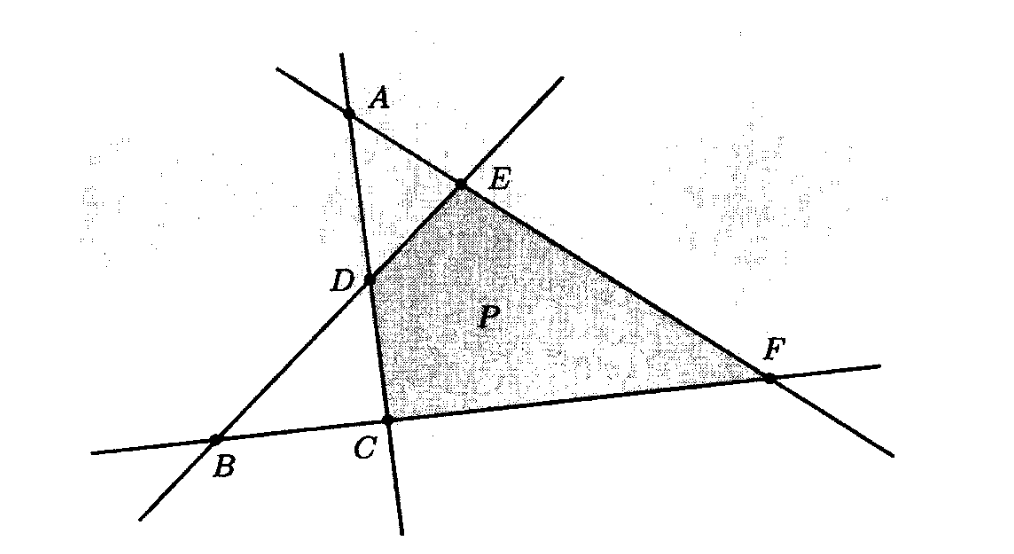
\includegraphics[width=0.5\textwidth]{fig/BT-fig2.7.png}
    \caption{Figure~2.7 in {\em Introduction To Linear Optimization} by Bertsekas and Tsitsiklis. The figure illustrates a polyhedral set $P\subset\rr^2$ where $A, B, C, D, E, F$ are all basic solutions to $P$ but only $C, D, E, F$ are basic feasible solutions. Every pair on the same line is a pair of adjacent basic solutions to $P$. }
    \label{fig: basic solution and adjacency}
\end{figure}

We should remind reader junior readers that the term ``basic'' stands for the adjective for ``basis'', which states that the solution is generated by a chosen linear algebraic basis. Observe that these two definitions, and the definition for an extreme point, are the same object in three different aspects. Before unifying the three characterizations of a polyhedral corner, it is worth reflecting on the logical architecture of our exposition. In Chapter~\ref{chapter: polyhedral geometry}, we established the fundamental equivalence between extreme points and basic feasible solutions ($\text{extreme point} \iff \text{basic feasible solution}$). This ordering is both deliberate and necessary: extreme points (geometric/topological) and basic feasible solutions (algebraic/algorithmic) are intrinsic to the polyhedron $P$ itself, depending solely on its defining constraint system without reference to an objective function. By isolating this intrinsic geometry-to-algebra bridge first in Theorem~\ref{thm: extreme points part 1}, we established a constructive computational skeleton for $P$. In this section, we introduce the extrinsic optimization perspective: the notion of a vertex defined relative to an optimization objective $\inner{\bmc, \cdot}$; and close the loop to synthesize all three viewpoints into one unified equivalence

\begin{theorem}
For a polyhedral set $P\subset \rr^{n}$ and a point $\bmx\rast \in \rr^{n}$. The following are equivalent. 
\begin{itemize}[noitemsep]
\item The point $\bmx\rast$ is a vertex in $P$. 
\item The point $\bmx\rast$ is an extreme point in $P$. 
\item The point $\bmx\rast$ is a basic feasible solution to $P$. 
\end{itemize}
\end{theorem}
\begin{proof}
Observe that Theorem~\ref{thm: extreme points part 1} is the proof for the point being an extreme point if and only if it is a basic feasible solution to $P$. We first show that a point $\bmx\rast$ is a vertex in $P$ implies that it is an extreme point in $P$; finally, we show that a point is a basic feasible solution to $P$ implies that it is a vertex in $P$. 

Suppose that $\bmx\rast\in P$ is a vertex. By definition, there exists $\bmc\in\rr^{n}$ such that for all $\bmx\in P\setminus\{\bmx\rast\}$, we have that $\inner{\bmc, \bmx\rast} > \inner{\bmc, \bmx}$. This says, for any two other points $\bmu, \bmw\in P$ and any $\alpha \in (0, 1)$, we have that 
\[ \inner{\bmc, \bmx\rast} > \alpha \inner{\bmc, \bmu}  + (1-\alpha) \inner{\bmc, \bmw}. \] 
Thus, there are no lines with endpoints in $P$ that contain $\bmx\rast$. 

Suppose that $\bmx\rast\in P$ is a basic feasible solution to $P$. Without loss of generality, we may assume $\bma_1, \bma_2, \dots, \bma_r$ are linear independent active constraints so that $\inner{\bma_j, \bmx\rast} = b_j$ that attains the bounds $b_j$, for $j\in\{1, 2, \dots, r\}$. We define a vector $\bmc = \sum_{i = 1}^m \bma_j$. Since the constraints are active, we have that  $\inner{\bmc, \bmx\rast} = \sum_{i = 1}^m  b_j$. By the linear indepdence, $\bmx\rast$ is the unique solution so that $\inner{\bma_j, \bmx\rast} = b_j$ for all $j\in\{1,2,\dots, r\}$ and, for any other $\bmx \in P\setminus\{\bmx\rast\}$, we have that $ \inner{\bma_j, \bmx\rast} > \inner{\bma_j, \bmx}$; this follows the definition of $\bmx\rast$ is a vertex in $P$. 
\end{proof}

%\begin{theorem}[Fundamental Theorem of Linear Programming]
%Consider the linear programming problem $\max_{\bmx} \inner{\bmc, \bmx}$ subject to $A\bmx\leq \bmb$, the optimal value $\bmx\rast$ occurs on the polyhedral set $\{\bmx: A\bmx = \bmb\}$. 
%\end{theorem}

%We remark on the choice of indices and rows; observe that $I_m = I_m^\top$. 
%\[A = \bmat{M\\ -M \\ -I_{m}} = 
%\left[\begin{array}{cccccc}
%| & | &  & | & & | \\ 
%\bmc_1& \bmc_2 & \dots & \bmc_k & \dots & \bmc_m\\
%| & | &  &| & & | \\ \hline
%| & | &  & | & & | \\ 
%-\bmc_1& -\bmc_2 & \dots & -\bmc_k & \dots & -\bmc_m\\
%| & | &  &| & & | \\ \hline
%| & | &  & | & & | \\ 
%-\bm\chi_1& -\bm\chi_2 & \dots & -\bm\chi_k & \dots & -\bm\chi_m\\
%| & | &  & | & & | \\ 
%\end{array}\right] 
%\]
%Next, we choose from $M$ a set of linearly independent rows, which are guaranteed by the fundamental theorem of linear algebra, and append a set of 
% 


